\documentclass{beamer}
\usepackage[utf8]{inputenc}
\usetheme{Madrid}
\usecolortheme{default}
\usepackage{amsmath,amssymb,amsfonts,amsthm}
\usepackage{txfonts}
\usepackage{tkz-euclide}
\usepackage{listings}
\usepackage{adjustbox}
\usepackage{array}
\usepackage{tabularx}
\usepackage{gvv}
\usepackage{lmodern}
\usepackage{circuitikz}
\usepackage{tikz}
\usepackage{graphicx}
\setbeamertemplate{page number in head/foot}[totalframenumber]
\usepackage{tcolorbox}
\tcbuselibrary{minted,breakable,xparse,skins}
\definecolor{bg}{gray}{0.95}
\DeclareTCBListing{mintedbox}{O{}m!O{}}{%
  breakable=true,
  listing engine=minted,
  listing only,
  minted language=#2,
  minted style=default,
  minted options={%
    linenos,
    gobble=0,
    breaklines=true,
    breakafter=,,
    fontsize=\small,
    numbersep=8pt,
    #1},
  boxsep=0pt,
  left skip=0pt,
  right skip=0pt,
  left=25pt,
  right=0pt,
  top=3pt,
  bottom=3pt,
  arc=5pt,
  leftrule=0pt,
  rightrule=0pt,
  bottomrule=2pt,
  toprule=2pt,
  colback=bg,
  colframe=orange!70,
  enhanced,
  overlay={%
    \begin{tcbclipinterior}
    \fill[orange!20!white] (frame.south west) rectangle ([xshift=20pt]frame.north west);
    \end{tcbclipinterior}},
  #3,
}
\lstset{
    language=C,
    basicstyle=\ttfamily\small,
    keywordstyle=\color{blue},
    stringstyle=\color{orange},
    commentstyle=\color{green!60!black},
    numbers=left,
    numberstyle=\tiny\color{gray},
    breaklines=true,
    showstringspaces=false,
}
\begin{document}

\title 
{4.11.37}
\date{september 15,2025}


\author 
{Namaswi-EE25BTECH11060}
\frame{\titlepage}
\begin{frame}{Question}
Show that the lines $\frac{x-1}{3}=\frac{y-1}{-1}=\frac{z+1}{0}$  and $\frac{x+4}{2}=\frac{y}{0}=\frac{z+1}{3}$ intersect.Find their point of intersection
\end{frame}
\begin{frame}{Lines}
  Let,
\begin{align}
\frac{x-1}{3}=\frac{y-1}{-1}=\frac{z+1}{0}=\lambda\\
\frac{x+4}{2}=\frac{y}{0}=\frac{z+1}{3}=\mu
\end{align}  
\end{frame}
\begin{frame}{Solution}
    \begin{align}
     \begin{pmatrix}
         1 & 1 & -1 
     \end{pmatrix}+\lambda \begin{pmatrix}
         3 & -1 & 0
     \end{pmatrix}=\begin{pmatrix}
         -4 & 0 & -1 
     \end{pmatrix}+ \mu \begin{pmatrix}
         2 & 0 & 3
     \end{pmatrix}\\
     \implies \begin{pmatrix}
         3 & -2 \\ -1 & 0 \\ 0 & -3 
     \end{pmatrix}\begin{pmatrix}
         \lambda \\ \mu
     \end{pmatrix}=\begin{pmatrix}
         -5 \\ -1 \\ 0
     \end{pmatrix}\\
 \end{align}
\end{frame}
\begin{frame}{solution}
  Using gaussian elimination\\
 Argumented matrix\\
 \begin{align}
     \begin{bmatrix}
         3 & -2 &  | & -5 \\
         -1 & 0  & | & -1\\
         0 & -3 & | & 0 
     \end{bmatrix}
 \end{align}
 Apply the row operation \( R_2 \to 3R_2 + R_1 \):
\begin{align}
\begin{bmatrix}
3 & -2 & | & -5\\
0 & -2 & | & -8\\
0 & -3 & | & 0
\end{bmatrix}
\end{align}

Divide the second row by \(-2\):
\begin{align}
\begin{bmatrix}
3 & -2 & | & -5\\
0 & 1  & | & 4\\
0 & -3 & | & 0
\end{bmatrix}
\end{align}

\end{frame}
\begin{frame}{solution}
 Now eliminate using \(R_2\):  
\[
R_1 \to R_1 + 2R_2, 
\quad R_3 \to R_3 + 3R_2
\]

\begin{align}
\begin{bmatrix}
3 & 0 & | & 3\\
0 & 1 & | & 4\\
0 & 0 & | & 12
\end{bmatrix}
\end{align}
 The last row gives \(0 = 12\), which is a contradiction.  
Hence, the system is inconsistent and has \textbf{no solution}.  
Therefore, the two lines are skew and do not intersect.
\end{frame}
\begin{frame}[fragile]
\frametitle{C Code}
\begin{lstlisting}
 #include <stdio.h>
int main() {
    // Augmented matrix for the system:
    // 3λ - 2μ = -5
    // -λ      = -1
    // -3μ     = 0
    
    double A[3][3] = {
        {3, -2, -5},
        {-1, 0, -1},
        {0, -3, 0}
    };
   
\end{lstlisting}
\end{frame}
\begin{frame}[fragile]
    \frametitle{C Code }
    \begin{lstlisting}
     // Perform Gaussian elimination
    for (int i = 0; i < 3; i++) {
        // Normalize row i if pivot nonzero
        if (A[i][i] != 0) {
            double pivot = A[i][i];
            for (int j = i; j < 3; j++) {
                A[i][j] /= pivot;
            }
        }
   // Eliminate column i from other rows
        for (int k = 0; k < 3; k++) {
            if (k != i) {
                double factor = A[k][i];
                for (int j = i; j < 3; j++) {
                    A[k][j] -= factor * A[i][j];
                }
            }
        }
    }

\end{lstlisting}
\end{frame}
\begin{frame}[fragile]
\frametitle{C Code }
\begin{lstlisting}
// After elimination, check last row
    if (A[2][0] == 0 && A[2][1] == 0 && A[2][2] != 0) {
        printf("System is inconsistent -> No solution. Lines are skew.\n");
    } else {
        double lambda = A[0][2];
        double mu = A[1][2];
        printf("Solution: lambda = %.2f, mu = %.2f\n", lambda, mu);
    }

    return 0;
}

\end{lstlisting}
\end{frame}
\begin{frame}[fragile]
\frametitle{Python Code}
\begin{lstlisting}
import numpy as np
import matplotlib.pyplot as plt

# Parameter range
t = np.linspace(-5, 5, 100)

# Line L1: (x,y,z) = (1,1,-1) + λ(3,-1,0)
x1 = 1 + 3*t
y1 = 1 - t
z1 = -1 * np.ones_like(t)

# Line L2: (x,y,z) = (-4,0,-1) + μ(2,0,3)
x2 = -4 + 2*t
y2 = np.zeros_like(t)
z2 = -1 + 3*t

\end{lstlisting}
\end{frame}

\begin{frame}[fragile]
\frametitle{Python Code}
\begin{lstlisting}
# Create 3D plot
fig = plt.figure(figsize=(8,6))
ax = fig.add_subplot(111, projection='3d')

# Plot the two lines
ax.plot(x1, y1, z1, label="Line L1: (1,1,-1)+λ(3,-1,0)", color='blue')
ax.plot(x2, y2, z2, label="Line L2: (-4,0,-1)+μ(2,0,3)", color='red')

# Mark given points
ax.scatter(1, 1, -1, color='blue', s=50, marker='o')
ax.text(1, 1, -1, "(1,1,-1)", color='blue')
\end{lstlisting}
\end{frame}
\begin{frame}[fragile]
    \frametitle{Python Code}
    \begin{lstlisting}
ax.scatter(-4, 0, -1, color='red', s=50, marker='o')
ax.text(-4, 0, -1, "(-4,0,-1)", color='red')

# Labels and title
ax.set_xlabel("X-axis")
ax.set_ylabel("Y-axis")
ax.set_zlabel("Z-axis")
ax.set_title("Skew Lines in 3D")
ax.legend()

plt.show()

\end{lstlisting}
\end{frame}
\begin{frame}[fragile]
\frametitle{C and Python Code}
\begin{lstlisting}
import ctypes

# Load the shared object file
lib = ctypes.CDLL('./skew.so')

# Call the function
result = lib.check_intersection()

if result == 0:
    print("System is inconsistent -> Lines are skew (no intersection).")
else:
    print("Lines intersect.")

\end{lstlisting}
\end{frame}

\begin{frame}{Plot}
    \centering
    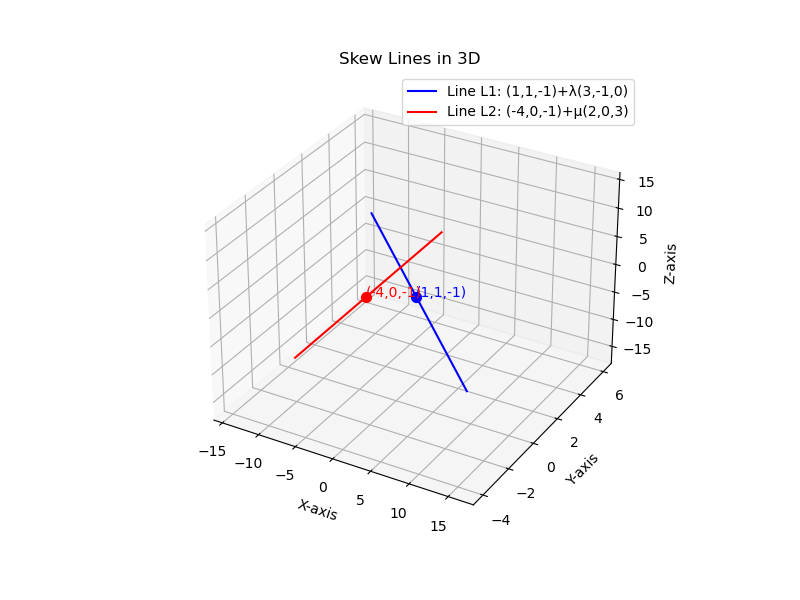
\includegraphics[width=\columnwidth, height=0.8\textheight, keepaspectratio]{Figure_8.png}     
\end{frame}
\end{document}